\documentclass{article}
% Para poder escribir las tildes directamente
\usepackage[utf8]{inputenc}
\usepackage[T1]{fontenc}
\usepackage[a4paper, total={6in, 8in}]{geometry}
\usepackage{amsmath, amssymb, amsthm}
\usepackage{cancel}
\usepackage{color,soul}
\usepackage[table,xcdraw]{xcolor}
\usepackage{comment}
\usepackage{graphicx}
\usepackage{hyperref}
\usepackage{listings}
\usepackage{outlines}
\usepackage{tcolorbox}
\usepackage{subcaption}
\usepackage[shortlabels]{enumitem}

% Para generar un nuevo environment de multicolumnas
% Creditos: https://tinyurl.com/5hbnu4wv
\usepackage{etoolbox,refcount}
\usepackage{multicol}

\newcounter{countitems}
\newcounter{nextitemizecount}
\newcommand{\setupcountitems}{%
  \stepcounter{nextitemizecount}%
  \setcounter{countitems}{0}%
  \preto\item{\stepcounter{countitems}}%
}
\makeatletter
\newcommand{\computecountitems}{%
  \edef\@currentlabel{\number\c@countitems}%
  \label{countitems@\number\numexpr\value{nextitemizecount}-1\relax}%
}
\newcommand{\nextitemizecount}{%
  \getrefnumber{countitems@\number\c@nextitemizecount}%
}
\newcommand{\previtemizecount}{%
  \getrefnumber{countitems@\number\numexpr\value{nextitemizecount}-1\relax}%
}
\makeatother    
\newenvironment{AutoMultiColItemize}{%
\ifnumcomp{\nextitemizecount}{>}{3}{\begin{multicols}{2}}{}%
\setupcountitems\begin{itemize}}%
{\end{itemize}%
\unskip\computecountitems\ifnumcomp{\previtemizecount}{>}{3}{\end{multicols}}{}}
%--------------------------------------------------

\title{Arquitectura de Computadoras}
\author{Nicolás Margenat}
\date{1Q 2022}

\begin{document}

\maketitle
\tableofcontents

\newpage
\section{Compilación}
\subsection{GCC Flags}
\begin{table}[h]
\centering
\begin{tabular}{|c|c|lll}
\cline{1-2}
\cellcolor[HTML]{84EE2F}{\color[HTML]{000000} Flags} & \cellcolor[HTML]{84EE2F}{\color[HTML]{000000} Descripción}                                                               &                      &  &  \\ \cline{1-2}
-c                                                   & compila y no linkedita                                                                                                   &                      &  &  \\ \cline{1-2}
-m32                                                 & \begin{tabular}[c]{@{}c@{}}le indica a gcc que genere archivo con formato\\ elf para arquitectura de 32bits\end{tabular} & \multicolumn{1}{c}{} &  &  \\ \cline{1-2}
-o \$1                                               & renombra el archivo de output a \$1                                                                                      &                      &  &  \\ \cline{1-2}
-fno-exceptions                                      & no te tira excepciones                                                                                                   &                      &  &  \\ \cline{1-2}
-S                                                   & te genera el file .asm                                                                                                   &                      &  &  \\ \cline{1-2}
-masm=intel                                          & \begin{tabular}[c]{@{}c@{}}es para que el -S te devuelva el .asm con\\ flavour de Intel\end{tabular}                     &                      &  &  \\ \cline{1-2}
\end{tabular}
\end{table}


\subsection{NASM Flags}
\begin{table}[h]
\centering
\begin{tabular}{|c|c|}
\hline
\rowcolor[HTML]{00D2CB} 
{\color[HTML]{000000} Flags} & {\color[HTML]{000000} Descripcion}                                                                                        \\ \hline
-f elf32                     & \begin{tabular}[c]{@{}c@{}}le indica a nasm que genere el file en formato\\ elf para arquitectura de 32 bits\end{tabular} \\ \hline
-f elf64                     & \begin{tabular}[c]{@{}c@{}}le indica a nasm que genere el file en formato\\ elf para arquitectura de 64 bits\end{tabular} \\ \hline
\end{tabular}
\end{table}

\begin{tcolorbox}[title=Compilación de archivo C y ASM]
\begin{verbatim}
> nasm -f elfXX $1.asm -o $1.o
> gcc -c -mXX $2.c -o $2.o
> gcc -mXX $1.o $2.o -o $3 
\end{verbatim}
donde XX es la arquitectura para la que generamos el archivo (32 o 64 bits).
\end{tcolorbox}

\begin{tcolorbox}[title=Compilación archivos ASM 32bits]
\begin{verbatim}
> nasm -f elf32 $1.asm -o $1.o
> ld -melf_i386 $1.o -o $1
\end{verbatim}
\end{tcolorbox}

%-------------
\newpage
\section{ASM}
\subsection{Sections}
\begin{enumerate}
    \item .rodata : datos constantes, inalterables
    \item .data : reserva espacio
    \item .bss : reserva espacio que no se aloca si no se usa
    \item .text : zona de código
\end{enumerate}

\subsection{Stack}
Como se ve el stack al llamar una función de ASM:
\begin{table}[h]
\centering
\begin{tabular}{|l|l|}
\hline
ESP           & Cantidad de argumentos                  \\ \hline
ESP + 4       & Path al programa                        \\ \hline
ESP + 8       & Dirección del 1er argumento             \\ \hline
ESP + 12      & Dirección del 2do argumento             \\ \hline
ESP + 16      & Dirección del 3er argumento             \\ \hline
ESP + (n+1)*4 & Dirección del n-argumento               \\ \hline
\rowcolor[HTML]{FFCCC9} 
              & NULL (4 bytes)                          \\ \hline
              & Dirección de la 1er variable de entorno \\ \hline
              & Dirección de la 2da variable de entorno \\ \hline
              & Dirección de la 3er variable de entorno \\ \hline
              & Dirección de la n-variable de entorno   \\ \hline
\rowcolor[HTML]{FFCCC9} 
              & NULL (4 bytes)                          \\ \hline
\end{tabular}
\end{table}
\\Una manera rápida de \emph{armar y desarmar el stack} es usando las macros: \texttt{enter} y \texttt{leave}.

\subsection{Registros}
\begin{table}[h]
\centering
\begin{tabular}{|c|c|c|c|c|}
\hline
\rowcolor[HTML]{FFD43F} 
\cellcolor[HTML]{FFC702}Registro    & AL/AH & AX   & EAX   & RAX   \\ \hline
\cellcolor[HTML]{FFCB2F}Size(bytes) & 1     & 2    & 4     & 8     \\ \hline
\cellcolor[HTML]{FFCB2F}Designation & Byte  & Word & DWord & QWord \\ \hline
\end{tabular}
\end{table}

%------
\newpage
\section{ASM y C}
\subsection{Registros a preservar entre llamadas a funciones}
\begin{itemize}
    \begin{AutoMultiColItemize}
        \item EBX
        \item ESI
        \item EDI
        \item EBP
        \item ESP
  \end{AutoMultiColItemize}
\end{itemize}

\subsection{Parámetros de una función}
Según la arquitectura, el compilador pasa de manera diferente los argumentos de las funciones:
\begin{align*}
    32\text{ bits} &\Rightarrow \text{Stack} \\
    64\text{ bits} &\Rightarrow \text{1° Registros, 2° Stack}
\end{align*}
Los \textbf{registros} que se utilizan para pasar argumentos en 64 bits son (por convención de C):
\begin{itemize}
    \begin{AutoMultiColItemize}
        \item RDI
        \item RSI
        \item RDX
        \item R10
        \item R9
        \item R8
  \end{AutoMultiColItemize}
\end{itemize}

% NOTE TO SELF: Para que funcione el \tabular adentro de tcolorbox no tenes que poner el env de table
\begin{tcolorbox}[title=Ejemplo (en C)]
Si en C tenemos:
\begin{verbatim}
    foo(paramA, paramB, paramC);
\end{verbatim}
se pushea en el stack de derecha a izquierda, de manera que queda:

\leavevmode\\
\centering
\begin{tabular}{|c|c|}
\hline
\textasciicircum{} & Dirección de retorno \\ \cline{2-2} 
| & paramA \\ \cline{2-2} 
| & paramB \\ \cline{2-2} 
| & paramC \\ \hline
\end{tabular}

\end{tcolorbox}

\subsection{Valores a retornar}
Si el valor es $\leq$ 32bits se retorna en EAX.
\\Si el valor es > 32bits se retorna la parte alta en EDX y la parte baja en EAX.
\\Si es un dato más complejo retorna un puntero formado por $\underbrace{\text{EDX}}_{\text{segmento}}:\underbrace{\text{EAX}}_{\text{offset}}$.

\newpage
\subsection{StackFrame}
Para armar (y desarmar) el StackFrame hacemos:
\begin{verbatim}
    push ebp        ; Armado de SF
    mov ebp, esp    ;
    ...
    ; codigo
    ...
    mov esp, ebp    ; Desarmado de SF
    pop ebp         ; 
\end{verbatim}

Finalmente, la pila terminaría pareciéndose a esto:
\begin{center}
    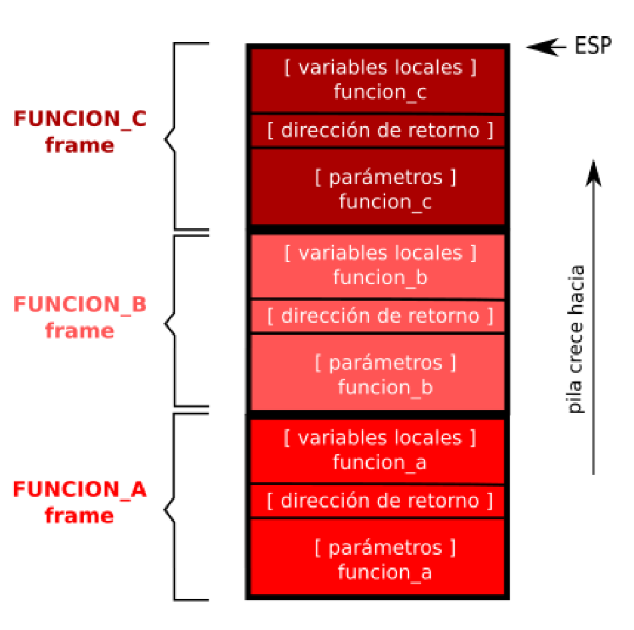
\includegraphics[width=.40\textwidth]{Images/StackFrame.png}
\end{center}   
%-----
\newpage
\section{Links útiles}
\subsection{Syscall IDs}
\underline{Arquitectura de 32bits}: \url{https://tinyurl.com/mpj5kxbw}
\\\underline{Arquitectura de 64bits}: \url{https://tinyurl.com/53khdbsv}

\end{document}
